\section{Zeitdiskrete Systeme}
\subsection{Elementare Zeitdiskrete Signale}
\begin{mdframed}[style=exercise]
	\begin{itemize}
		\item \textbf{Einheitsimpulse}\\
		      \makebox[\textwidth][c]
		      {
			      \begin{minipage}{0.3\textwidth}
				      \[
					      \delta(n) =
					      \begin{cases}
						      1 & n = 0    \\
						      0 & n \neq 0
					      \end{cases}
				      \]
			      \end{minipage}
			      \begin{minipage}{0.7\textwidth}
				      \centering
				      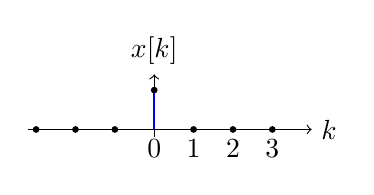
\begin{tikzpicture}[baseline=0.8,scale=0.5]
					      \draw[->] (0,-0.2) -- (0,1.4) node[above]{$x[k]$}; %y
					      \draw[->] (-3.2,0) -- (4,0) node[right]{$k$}; %x
					      \filldraw[black] (-3,0) circle (2pt) {};
					      \filldraw[black] (-2,0) circle (2pt) {};
					      \filldraw[black] (-1,0) circle (2pt) {};
					      \draw[blue, thick] (0,1) -- (0,0) node[below, black]{0}; \filldraw[black] (0,1) circle (2pt) {};
					      \filldraw[black] (1,0) circle (2pt) node[below]{1};
					      \filldraw[black] (2,0) circle (2pt) node[below]{2};
					      \filldraw[black] (3,0) circle (2pt) node[below]{3};
				      \end{tikzpicture}
			      \end{minipage}
		      }
		      Eigenschaften:
		      \begin{itemize}
			      \item neutrales Element der Faltung
			      \item Anregung der Impulsantwort
			      \item besitzt konstantes Spektrum
			      \item Summe ist $\sum^{\infty}_{n=-\infty}\delta(n)=1$
		      \end{itemize}
		      Ausblendeeigenschaft:
		      \[
			      x(n) = \sum_{k=-\infty}^{\infty} x(k)\cdot\delta(n-k)
		      \]
		\item \textbf{Einheitssprung}\\
		      \makebox[\textwidth][c]
		      {
			      \begin{minipage}{0.3\textwidth}
				      \[
					      \varepsilon(n) =
					      \begin{cases}
						      1 & n \geq 0 \\
						      0 & n < 0
					      \end{cases}
				      \]
			      \end{minipage}
			      \begin{minipage}{0.7\textwidth}
				      \centering
				      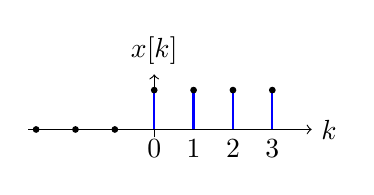
\begin{tikzpicture}[baseline=0.8,scale=0.5]
					      \draw[->] (0,-0.2) -- (0,1.4) node[above]{$x[k]$}; %y
					      \draw[->] (-3.2,0) -- (4,0) node[right]{$k$}; %x
					      \filldraw[black] (-3,0) circle (2pt) {};
					      \filldraw[black] (-2,0) circle (2pt) {};
					      \filldraw[black] (-1,0) circle (2pt) {};
					      \draw[blue, thick] (0,1) -- (0,0) node[below, black]{0}; \filldraw[black] (0,1) circle (2pt) {};
					      \draw[blue, thick] (1,1) -- (1,0) node[below, black]{1}; \filldraw[black] (1,1) circle (2pt) {};
					      \draw[blue, thick] (2,1) -- (2,0) node[below, black]{2}; \filldraw[black] (2,1) circle (2pt) {};
					      \draw[blue, thick] (3,1) -- (3,0) node[below, black]{3}; \filldraw[black] (3,1) circle (2pt) {};
				      \end{tikzpicture}
			      \end{minipage}
		      }
		      Zusammenhang mit Einheitsimpulse:
		      \[
			      \delta(n) = \varepsilon(n) - \varepsilon(n-1)
		      \]
		\item \textbf{Rechteckfolge}\\
		      \makebox[\textwidth][c]
		      {
			      \begin{minipage}{0.3\textwidth}
				      \[
					      \operatorname{rect}(n) =
					      \begin{cases}
						      1 & 0 \leq n < N   \\
						      0 & \texttt{sonst}
					      \end{cases}
				      \]
			      \end{minipage}
			      \begin{minipage}{0.7\textwidth}
				      \centering
				      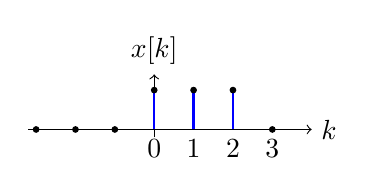
\begin{tikzpicture}[baseline=0.8,scale=0.5]
					      \draw[->] (0,-0.2) -- (0,1.4) node[above]{$x[k]$}; %y
					      \draw[->] (-3.2,0) -- (4,0) node[right]{$k$}; %x
					      \filldraw[black] (-3,0) circle (2pt) {};
					      \filldraw[black] (-2,0) circle (2pt) {};
					      \filldraw[black] (-1,0) circle (2pt) {};
					      \draw[blue, thick] (0,1) -- (0,0) node[below, black]{0}; \filldraw[black] (0,1) circle (2pt) {};
					      \draw[blue, thick] (1,1) -- (1,0) node[below, black]{1}; \filldraw[black] (1,1) circle (2pt) {};
					      \draw[blue, thick] (2,1) -- (2,0) node[below, black]{2}; \filldraw[black] (2,1) circle (2pt) {};
					      \filldraw[black] (3,0) circle (2pt) node[below] {3};
				      \end{tikzpicture}
			      \end{minipage}
		      }
		      Zusammenhang mit Dirac- und Einheitsimpuls:
		      \begin{align*}
			      \operatorname{rect}(n) & = \varepsilon(n) + \varepsilon(n-N)       \\
			                             & = \varepsilon(n) \cdot \varepsilon(N-1-n)
		      \end{align*}
		\item \textbf{Zeitdiskrete Sinus}\\
		      \makebox[\textwidth][c]
		      {
			      \begin{minipage}{0.3\textwidth}
				      \[
					      x(n) = A \cdot \sin(\Omega n+\varphi)
				      \]
			      \end{minipage}
			      \begin{minipage}{0.7\textwidth}
				      \centering
				      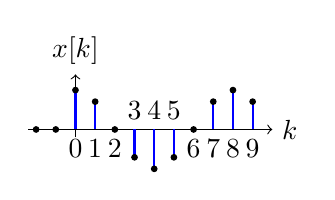
\begin{tikzpicture}[baseline=1,scale=0.5]
					      \draw[->] (0,-0.2) -- (0,1.4) node[above]{$x[k]$}; %y
					      \draw[->] (-1.2,0) -- (5,0) node[right]{$k$}; %x
					      \filldraw[black] (-1,0) circle (2pt) {};
					      \filldraw[black] (-0.5,0) circle (2pt) {};
					      \draw[blue,thick] (0,1) -- (0,0)          node[below, black]{0}; \filldraw[black] (0,1) circle (2pt) {};
					      \draw[blue,thick] (0.5,0.707) -- (0.5,0)  node[below, black]{1}; \filldraw[black] (0.5,0.707) circle (2pt) {};
					      \filldraw[black] (1,0) circle (2pt)              node[below, black]{2};
					      \draw[blue,thick] (1.5,-0.707) -- (1.5,0) node[above, black]{3}; \filldraw[black] (1.5,-0.707) circle (2pt) {};
					      \draw[blue,thick] (2,-1) -- (2,0)         node[above, black]{4}; \filldraw[black] (2,-1) circle (2pt) {};
					      \draw[blue,thick] (2.5,-0.707) -- (2.5,0) node[above, black]{5}; \filldraw[black] (2.5,-0.707) circle (2pt) {};
					      \filldraw[black] (3,0) circle (2pt)              node[below]{6};
					      \draw[blue,thick] (3.5,0.707) -- (3.5,0)  node[below, black]{7}; \filldraw[black] (3.5,0.707) circle (2pt) {};
					      \draw[blue,thick] (4,1) -- (4,0)          node[below, black]{8}; \filldraw[black] (4,1) circle (2pt) {};
					      \draw[blue,thick] (4.5,0.707) -- (4.5,0)  node[below, black]{9}; \filldraw[black] (4.5,0.707) circle (2pt) {};
				      \end{tikzpicture}
			      \end{minipage}
		      }
		      \footnotesize
		      \begin{align*}
			      A       & :\texttt{Amplitude}               \\
			      \Omega  & :\texttt{normierte Kreisfrequenz} \\
			      \varphi & :\texttt{Anfangsphase}
		      \end{align*}
		      \normalsize
		\item \textbf{Exponentialfolge}\\
		      \makebox[\textwidth][c]
		      {
			      \begin{minipage}{0.3\textwidth}
				      \begin{align*}
					      x(n) & = \underline{A} \cdot e^{Sn}                \\
					           & = \underline{A} \cdot e^{(\Sigma+j\Omega)n}
				      \end{align*}
			      \end{minipage}
			      \begin{minipage}{0.7\textwidth}
				      \centering
				      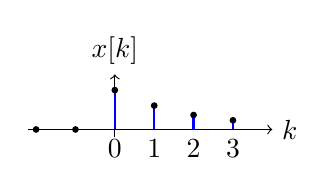
\begin{tikzpicture}[baseline=0.8,scale=0.5]
					      \draw[->] (0,-0.2) -- (0,1.4) node[above]{$x[k]$}; %y
					      \draw[->] (-2.2,0) -- (4,0) node[right]{$k$}; %x
					      \filldraw[black] (-2,0) circle (2pt) {};
					      \filldraw[black] (-1,0) circle (2pt) {};
					      \draw[blue, thick] (0,1) -- (0,0) node[below, black]{0}; \filldraw[black] (0,1) circle (2pt) {};
					      \draw[blue, thick] (1,0.606) -- (1,0) node[below, black]{1}; \filldraw[black] (1,0.606) circle (2pt) {};
					      \draw[blue, thick] (2,0.367) -- (2,0) node[below, black]{2}; \filldraw[black] (2,0.367) circle (2pt) {};
					      \draw[blue, thick] (3,0.233) -- (3,0) node[below, black]{3}; \filldraw[black] (3,0.233) circle (2pt) {};
				      \end{tikzpicture}
			      \end{minipage}
		      }
		      \begin{align*}
			      S                                       & = \Sigma+j\Omega        \\
			      \texttt{Amplitudenänderung }\Sigma      & = \sigma T = \sigma/f_A \\
			      \texttt{normierte Kreisfrequenz }\Omega & = \omega T =  2\pi f_A
		      \end{align*}
	\end{itemize}
\end{mdframed}
\subsection{Abtasttheorem im Fequenzbereich}
Nur wenn das Eingangssignal auf $\omega_g$ bandbegrenzt und die Abtastfrequenz $\omega_a  \geq
	2\omega_g$ ist, kommt es nicht zu spektralen Überlappungen (= Aliasing).

Aliasing führt zu zusätzlichen Abtastwerten nicht mehr rekonstruieren lässt.

\centering
\includegraphics[width=0.5\columnwidth]{Bilder/Abtasttheorem_Uebrlappung}

\raggedright
\vspace{-1.5em}
\subsection{Elementare Zeitdiskrete Systeme}
\subsubsection{Definition}
Ein System, das sowohl linear, als auch zeitinvariant ist, nennen wir ein
lineares zeitinvariantes System, oder kurz LTI-System

\subsubsection{Kausalität und Stabilität}
\begin{itemize}
	\item \textbf{Kausal}:
	      wenn die Anzahl der Pole (Grad des Nenners) größer gleich
	      der Anzahl der Nullstellen (Grad des Zählers) ist.
	      $ h(n) = 0 \texttt{ für } n<0 $
	\item \textbf{Stabil}:
	      wenn der Einheitskreis zum Konvergenzbereich gehört
	      $ \sum_{n=-\infty}^{\infty}|h(n))| < \infty $
\end{itemize}

\begin{center}
	\fbox{\parbox{.9\columnwidth}{Liegen alle Pole innerhalb des Einheitskreises,
			so ist das LTI-System kausal und stabil!}}
\end{center}

\subsubsection{Faltung}

\vspace{1ex}
Beispiel Impulsantworttabelle:
\vspace{-1em}
\begin{center}
	\begin{table}[H]
		\footnotesize
		\centering
		\begin{tabular}{|c|cccc|c|ccc|}
			\hline
			  & $d_0$ & $d_1$ & $d_2$ & $d_3$ & $\frac{1}{c_0}$               & $c_1$    & $c_2$ & $c_3$ \\
			\hline
			k & 0     & 1     & 0     & -1    & $h[k]$                        & 0        & -0,25 & 0     \\
			\hline
			0 & 1     &       &       &       &                               &          &       &       \\
			\hline
			1 &       & 1     &       &       & 1                             &          &       &       \\
			\hline
			2 &       &       & 1     &       &                               & 1        &       &       \\
			\hline
			3 &       &       &       & 1     & $1 \cdot 1 + (-0,25) \cdot 1$ &          & 1     &       \\
			\hline
			4 &       &       &       &       &                               & $-1,25 $ &       & 1     \\
			\hline
			5 &       &       &       &       & $-1,25/4$                     &          & -1,25 &       \\
			\hline
		\end{tabular}
	\end{table}

	\includegraphics[width=0.4\columnwidth]{Bilder/Signalflussdiagramm}
\end{center}

Alternativ mit der Differenzengleichung:
\[
	\left.\underline{H}(z)=\frac{8 \cdot z^{2}-2 \cdot z-2}{z^{2}+0,25} = \frac{8 -2 \cdot z^1-2 \cdot z^{-2}}{1 + 0,25 \cdot z^{-2}}\right\} \frac{b}{a}=\frac{Y}{X}
\]
Differenzengleichung $\rightarrow y(n) = 8x(n) -2x(n-1)-2x(n-2)-0,25y(n-2)$
\begin{align*}
	\begin{split}
		a_{0} y(n)+a_{1} y(n-1)+\ldots+a_{N} y(n-N)=\\
		b_{0} x(n)+b_{1} x(n-1)+\ldots+b_{M} x(n-M)
	\end{split}
\end{align*}

\subsubsection{Signalflussplan / Signalflussgraph}

\includegraphics[width=\columnwidth]{Bilder/Signalfluss_plan-graph}

\begin{itemize}
	\item Ein Knoten, in den ein Zweig hinein und zwei oder mehr Zweige
	      hinausgehen, ist eine Verzweigung.
	\item Ein Knoten, in den mehrere Zweige hinein und ein Zweig hinausgeht,
	      ist ein Addierer.
	\item Ein Pfeil, über den ein Koeffizient geschrieben ist, beschreibt
	      eine Multiplikation des Signals mit dem Koeffizienten.
	\item Ein Zweig, über den $z^{-1}$ geschrieben ist, beschreibt eine
	      Verzögerung um einen Abtasttakt.
\end{itemize}

\subsubsection{Klassifizierung von Systemen}
% Die mathematischen Beschreibung fehlen. wurden nie gebraucht während lernen. Kap6S63 6.5.7
\begin{mdframed}[style=exercise]
	\begin{itemize}
		\item \textbf{Transversale Systeme:}\\
		      Der Ausgang wird nicht auf den Eingang zurückgeführt\\
		      $\Rightarrow$ $a_k=0 \texttt{ für } k>0$\\
		      $\Rightarrow$ alle Pole liegen im Ursprung

		      \makebox[\columnwidth][c]{
			      \begin{minipage}{0.4\textwidth}
				      \includegraphics[width=0.7\textwidth]{Bilder/Transversale_Systeme_}
			      \end{minipage}
			      \hspace{-1em}
			      \begin{minipage}{0.6\textwidth}
				      \includegraphics[width=0.8\textwidth]{Bilder/Transversale_Systeme_SG}
			      \end{minipage}
		      }
		\item \textbf{Rekursive Systeme:}\\
		      Der aktuelle Ausgangswert hängt nur vom aktuellen Eingangswert
		      und früheren Ausgangswerten ab.\\
		      $\Rightarrow$ $b_k=0 \texttt{ für } k>0$\\
		      $\Rightarrow$ alle Nullstellen liegen im Ursprung

		      \makebox[\columnwidth][c]{
			      \begin{minipage}{0.4\textwidth}
				      \includegraphics[width=0.7\textwidth]{Bilder/Rekursive_Systeme}
			      \end{minipage}
			      \hspace{-1em}
			      \begin{minipage}{0.6\textwidth}
				      \includegraphics[width=0.8\textwidth]{Bilder/Rekursive_Systeme_SG}
			      \end{minipage}
		      }
	\end{itemize}
\end{mdframed}

Systeme nach der Länge der Impulsantwort
\begin{itemize}
	\item \textbf{Finite Impulse Response (FIR) Systeme:}\\
	      \bulletptR haben \underline{endlich} lange Impulsantworten\\
	      \bulletptR synonym zum Begriff transversales System\\
	      \bulletptR endlich lange Impulsantworten lassen sich auch mit
	      transversal-rekursiven Systemen erreichen
	\item \textbf{Infinite Impulse Response (IIR) Systeme:}\\
	      \bulletptR haben \underline{unendlich} lange Impulsantworten\\
	      \bulletptR synonym zum Begriff rekursives System
\end{itemize}

\end{multicols*}

\subsection{s-Frequenzebene/z-Frequenzebene}
\begin{center}
	\begin{tabular}[htpb]{c|c|c}
		s-Frequenzebene     & $e^{sT} = z$          & z-Frequenzebene     \\
		\hline
		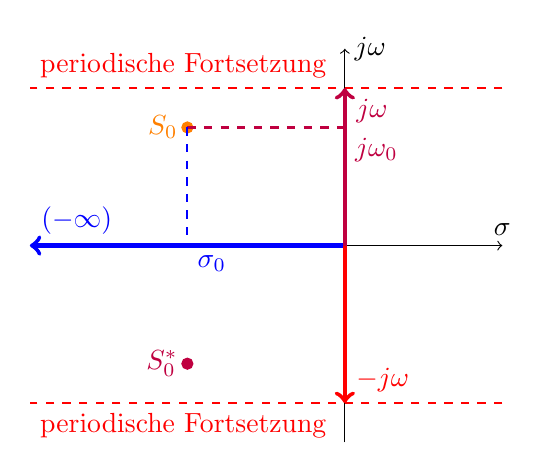
\begin{tikzpicture}[baseline=1]
    \draw[->] (0,-2.5) -- (0,2.5) node[right]{$j\omega$}; %y
    \draw[->] (-4,0) -- (2,0) node[above]{$\sigma$}; %x

    \draw[thick, dashed, red] (2,2) -- (-4,2) node[above right]{periodische Fortsetzung};
    \draw[thick, dashed, red] (2,-2) -- (-4,-2) node[below right]{periodische Fortsetzung};
    \draw[ultra thick, ->, blue] (0,0) -- (-4,0) node[above right]{$(-\infty)$};
    \draw[ultra thick, ->, purple] (0,0) -- (0,2) node[below right]{$j \omega$};
    \draw[ultra thick, ->, red] (0,0) -- (0,-2) node[above right]{$-j \omega$};

    \filldraw[orange] (-2,1.5) circle (2pt) node[left]{$S_0$};
    \draw[thick, dashed, purple] (-2,1.5) -- (0,1.5) node[below right]{$j \omega_0 $};
    \draw[thick, dashed, blue] (-2,1.5) -- (-2,0) node[below right]{$ \sigma_0 $};

    \filldraw[purple] (-2,-1.5) circle (2pt) node[left]{$S_0^*$};
\end{tikzpicture}
 & $\Longleftrightarrow$ & 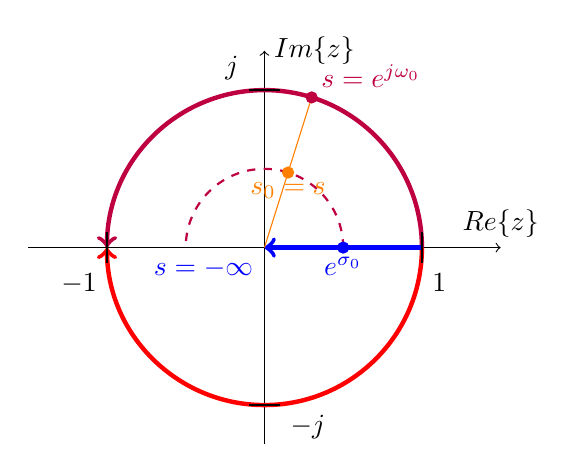
\begin{tikzpicture}[baseline=1]
    \draw[->] (0,-2.5) -- (0,2.5) node[right]{$\mathfrak{Im}\{z\}$}; %y
    \draw[->] (-3,0) -- (3,0) node[above]{$\mathfrak{Re}\{z\}$}; %x

    \draw[thick, color=black, dashed](0,0) circle (2);
    \draw[ultra thick, ->, purple] (2,0) arc (0:180:2);
    \draw[ultra thick, ->, red] (2,0) arc (0:-180:2);
    \draw[ultra thick, ->, blue] (2,0) -- (0,0) node[below left]{$s =-\infty$};

    \draw[thick, dashed, purple] (1,0) arc (0:180:1);

    \draw[thick, black] (0.2,2) -- (-0.2,2) node[above left]{$j$};
    \draw[thick, black] (-0.2,-2) -- (0.2,-2) node[below right]{$-j$};
    \draw[thick, black] (2,0.2) -- (2,-0.2) node[below right]{$1$};
    \draw[thick, black] (-2,0.2) -- (-2,-0.2) node[below left]{$-1$};

    \filldraw[blue] (1,0) circle (2pt) node[below]{$ e^{\sigma_0}$};
    \filldraw[orange] (0.3,0.953) circle (2pt) node[below]{$s_0 = s$};
    \draw[orange] (0,0) -- (0.6,1.907) {};
    \filldraw[purple] (0.6,1.907) circle (2pt) node[above right]{$s=e^{j \omega_0}$};
\end{tikzpicture}
 \\
	\end{tabular}
\end{center}

\begin{multicols*}{2}
\subsubsection{Zeitdiskrete Fouriertransformation}
\begin{mdframed}[style=exercise,]
	zeitdiskrete Fouriertransformation (DTFT):
	\[
		\underline{X}(\Omega) = \sum_{k=-\infty}^{\infty} x(k)e^{-j\Omega k}
	\]
	zeitdiskrete Fourier-Inverse-Transformation (IDTFT):
	\[
		\underline{x}(k) = \frac{1}{2\pi}\int_{\pi}^{\pi} X(\Omega)e^{j\Omega} d\Omega
	\]

	\footnotesize
	beide sind gleich: $x(n)=x(k)$
\end{mdframed}
\subsubsection{Z-Transformation}
\begin{mdframed}[style=exercise]
	Die LT von $x_a(t)$ ist gleich der z-Transformation von $x(k)$:
	$e^{sT}=z$
	\[
		\underline{X}(s) = \sum_{k=-\infty}^{\infty} x(kT)e^{-skT} \Rightarrow \underline{X}(z) = \sum_{k=-\infty}^{\infty} x(k)z^{-k}
	\]
\end{mdframed}
für die Rücktransformation wird Partialbruchzerlegung verwendet.
\[
	\underline{X}(z)=\frac{\underline{Z}(z)}{\underline{N}(z)}=\frac{\sum_{m=0}^{M} b_{m} z^{m}}{\sum_{n=0}^{N} a_{n} z^{n}}=\frac{b_{M}}{a_{N}} \cdot \frac{\prod_{m=1}^{M}\left(z-z_{o m}\right)}{\prod_{n=1}^{N}\left(z-z_{x n}\right)}
\]
bei einfachen Polstellen gilt:
\begin{align*}
	\Aboxed{\frac{\underline{X}(z)}{z} & =\frac{c_{0}}{z}+\frac{c_{1}}{z-z_{x 1}}+\frac{c_{2}}{z-z_{x 2}}+\cdots+\frac{c_{N}}{z-z_{x N}}} \\
	                                   & =\frac{c_{0}}{z}+\sum_{n=1}^{N} \frac{c_{n}}{z-z_{x n}}
\end{align*}
bei mehrfachen Polstellen gilt:
\begin{align*}
	\Aboxed{\frac{\underline{X}(z)}{z}=\frac{c_{0}}{z}+\frac{c_{1}}{z-z_{x n}}+\frac{c_{2}}{\left(z-z_{x n}\right)^{2}}+\cdots+\frac{c_{k}}{\left(z-z_{x n}\right)^{k}}}
\end{align*}

\subsubsection{Übertragungsfunktion $\Leftrightarrow$ Differenzengleichung}
\[
	\underline{H}(z)=\frac{\underline{Y}(z)}{\underline{X}(z)}=\frac{\sum_{k=0}^{M} b_{k} \cdot z^{-k}}{1+\sum_{k=1}^{N} a_{k} \cdot z^{-k}}=\frac{\sum_{k=0}^{M} b_{k} \cdot z^{N-k}}{z^{N}+\sum_{k=1}^{N} a_{k} \cdot z^{N-k}}
\]

\subsubsection{PN-Diagramm $\Rightarrow$ Frequenzebene}
\begin{mdframed}[style=exercise]
	$z=e^{j\Omega}$ bedeutet: um $\underline{H}(\Omega)$ zu ermittlen, muss man
	den Einheitskreis entlang gehen.
	\[
		\underline{H}(\Omega)=\left.\underline{H}(z)\right|_{z=e^{j \Omega}}
	\]
\end{mdframed}
Beispiel:
\[
	\underline{H}(z)=\frac{\left(z-z_{o}\right)}{\left(z-z_{x}\right)}
\]
\[
	\underline{H}(\Omega)=\frac{\left(e^{j \Omega}-z_{o}\right)}{\left(e^{j \Omega}-z_{x}\right)}=\frac{A_{o} e^{j \varphi_{o}}}{A_{x} e^{j \varphi_{x}}}
\]

\centering
\includegraphics[width=0.7\columnwidth]{Bilder/PN-FreqGang}

\raggedright
\textbf{Betragsfrequenzgang}
\[
	H(\Omega)=\frac{A_{o}(\Omega)}{A_{x}(\Omega)}
\]
\textbf{Phasenfrequenzgang}
\[
	\varphi_{H}(\Omega)=\varphi_{o}(\Omega)-\varphi_{x}(\Omega)
\]

Aus dem  Punkt (1,0) starten und am Einheitskreis entlang gegen den
Uhrzeigersinn gehen.
\makebox[\columnwidth][c]{
	\begin{minipage}{0.5\columnwidth}
		\begin{center}
			\includegraphics[width=0.9\columnwidth]{Bilder/PN-FreqGang_BSP-P1}
		\end{center}
	\end{minipage}
	\begin{minipage}{0.5\columnwidth}
		\begin{center}
			\includegraphics[width=0.8\columnwidth]{Bilder/PN-FreqGang_BSP-P2}
		\end{center}
	\end{minipage}
}
\makebox[\columnwidth][c]{
	\begin{minipage}{0.5\columnwidth}
		\begin{center}
			\includegraphics[width=0.9\columnwidth]{Bilder/PN-FreqGang_BSP1-P1}
		\end{center}
	\end{minipage}
	\begin{minipage}{0.5\columnwidth}
		\begin{center}
			\includegraphics[width=0.8\columnwidth]{Bilder/PN-FreqGang_BSP2-P2}
		\end{center}
	\end{minipage}
}
